\documentclass[10pt]{article}
\usepackage{parskip}
\usepackage[utf8]{inputenc}
\usepackage[left=2.00cm, right=2.00cm, top=2.00cm, bottom=2.00cm]{geometry}
\usepackage[spanish]{babel}
\usepackage{graphicx,subfig}
\usepackage{fancyhdr}
\graphicspath{{Imagenes/}}
\usepackage{enumerate} 
\usepackage{multicol}
\usepackage{tabularx}
\usepackage{amssymb}
\usepackage{adjustbox}
\usepackage{circuitikz}
\usepackage{amsmath}
\usepackage{cancel}
\begin{document}


\pagestyle{fancy}
\cfoot{}


%Cabeceras
\rhead{Práctica Leyes de Kirchhoff.}
\lhead{}

%Portada
\begin{titlepage}
	\newgeometry{
		left=25mm,
		right=25mm,
		top=5mm,
		bottom=30mm,
		headheight = 0 mm
	}

	\begin{figure}[t]
		\subfloat{
\includegraphics[width=0.15\textwidth]{Logo_IPN}}
		\hspace{0.6\textwidth}
		\subfloat{
\includegraphics[width=0.22\textwidth]{LogoEsime}}
	\end{figure}

	\centering
	{\bfseries\Huge Instituto Politécnico Nacional. \par}
	\vspace{1cm}
	{\scshape\Large Ingeniería en Comunicaciones y Electrónica. \par}
	\vspace{0.3cm}
	{\scshape\Large Laboratorio de Circuitos.  \par}
	\vspace{1cm}
	{\scshape\Huge Kirchhoff \par}
	\vspace{1cm}
	{\itshape\Large Práctica Leyes de Kirchhoff. \par}
	{\Large 3CM7\par}
	\vfill
	{\Large Autores: \par}
	{\Large José Emilio Hernández Huerta. \par}
	{\Large SERGIO SAMUEL REYES MORENO. \par}
	
	\vfill
	{\Large Octubre 2023. \par}

\end{titlepage}

\newpage


\subsection{Primera parte. Cálculos teóricos}

\begin{circuitikz}
    \draw (0,0) to[battery, v=9V, invert] (0,2)
        to[R, l=$R_1$, *-, R=$1k\Omega$] (2,2)
        to[R, l=$R_3$, -*, R=$1k\Omega$] (4,2)
        to[short] (6,2) % Aumenta el valor X para separar más el resistor 5
        to[R, l=$R_5$, -*, R=$1k\Omega$] (6,0)
        to[short] (0,0);
\draw (2,2) to[R, l=$R_2$, *-, R=$1k\Omega$] (2,0);
\draw (4,2) to[R, l=$R_4$, -*, R=$1k\Omega$] (4,0);



\end{circuitikz}

\begin{center}
	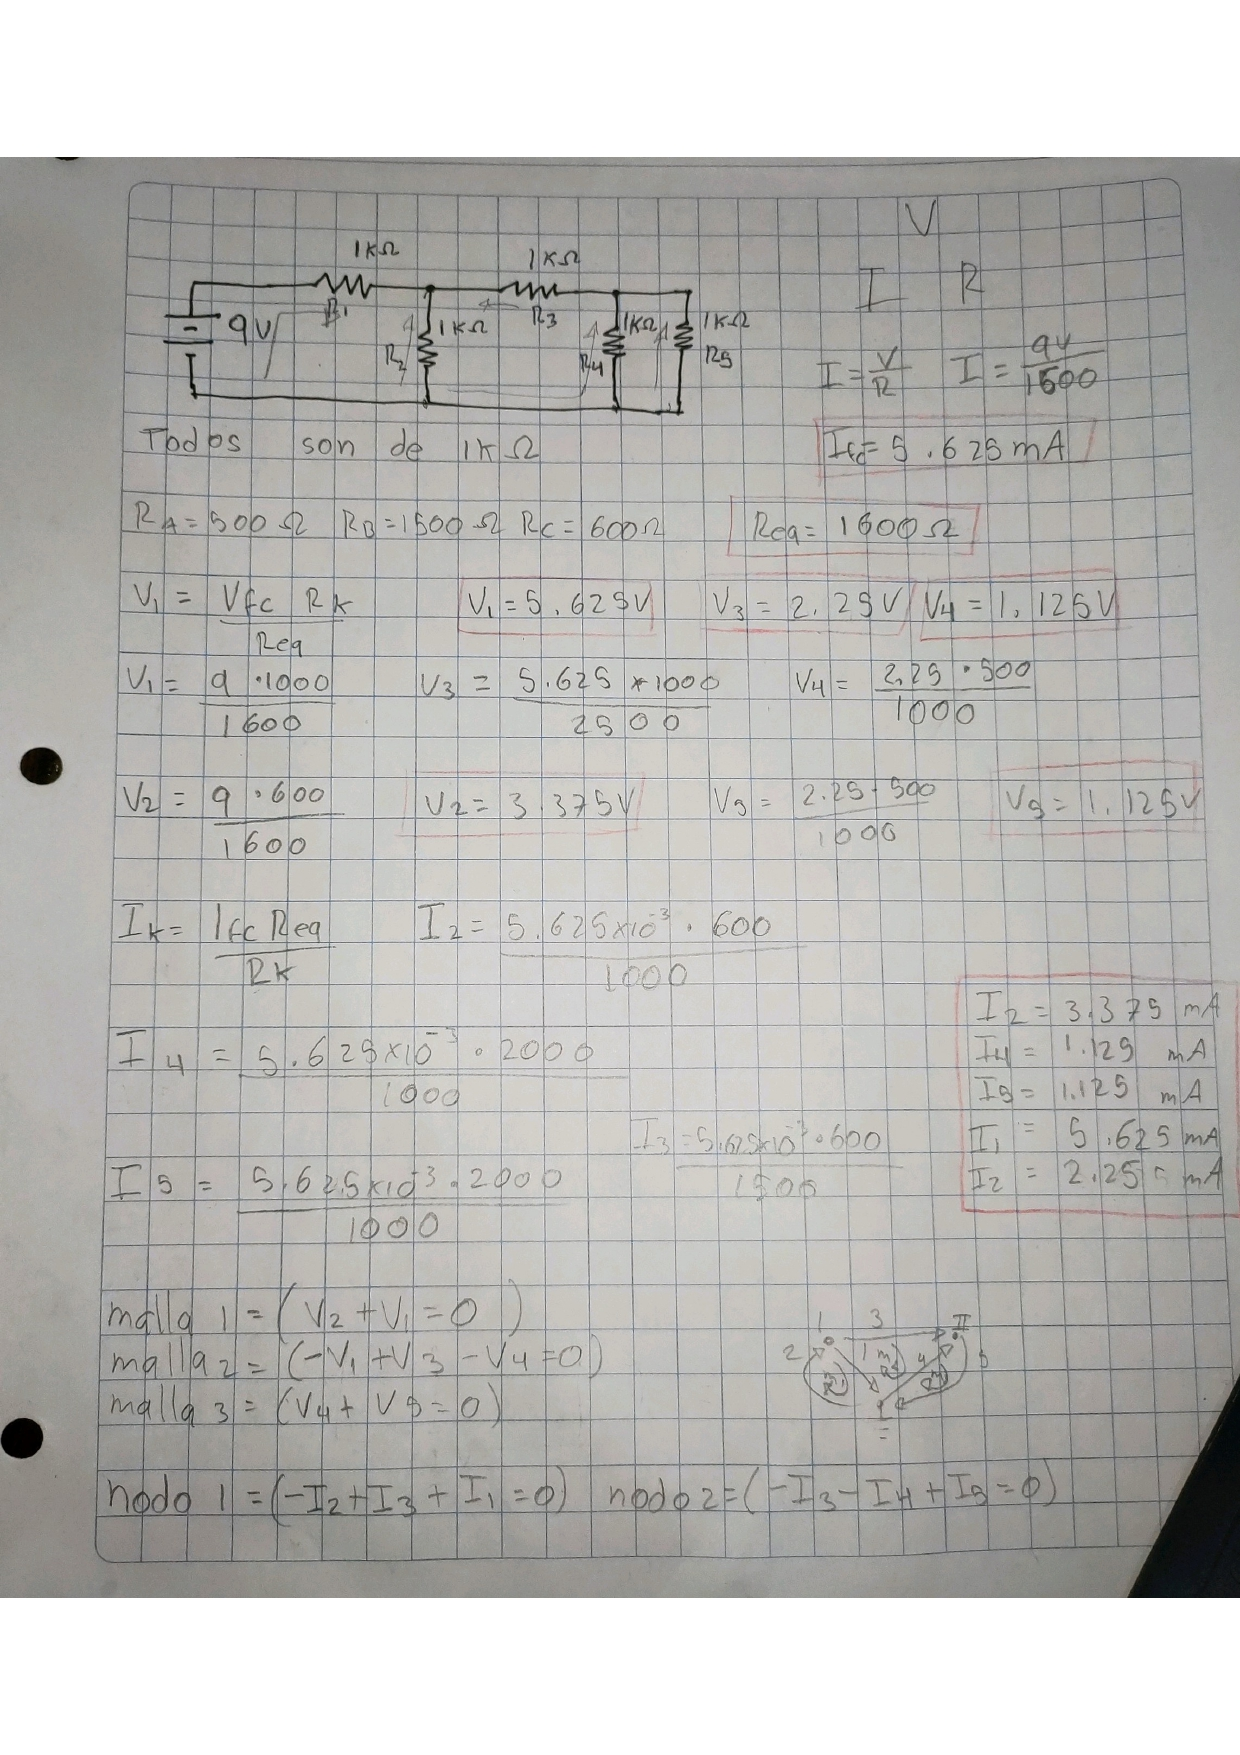
\includegraphics[width=14.5cm, height=18.86cm]{Imagenes/Calculos.jpg}
	\captionof{figure}{Calculos}
	
\end{center}
\newpage
    
\subsection{Segunda parte. Simulación}
\begin{center}
	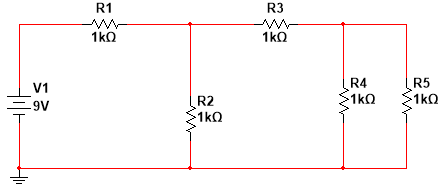
\includegraphics[width=8.075cm, height=3.791cm]{Imagenes/Circuito.png}
	\captionof{figure}{Circuito original.}
	
\end{center}
\begin{center}
	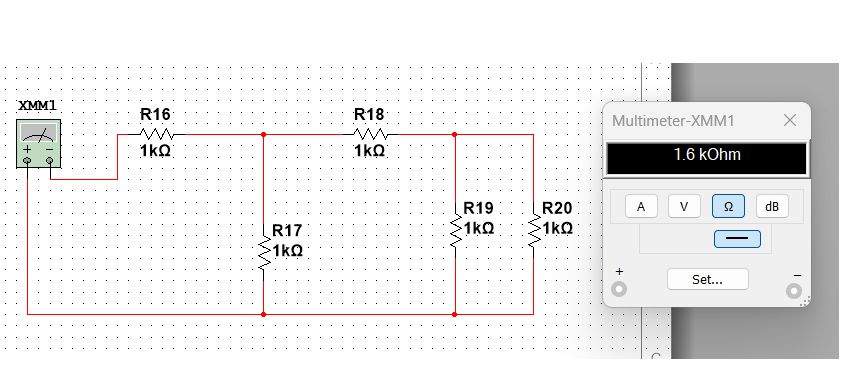
\includegraphics[width=8.075cm, height=3.791cm]{Imagenes/req.png}
	\captionof{figure}{Resistencia equivalente.}
\end{center}


\begin{center}
	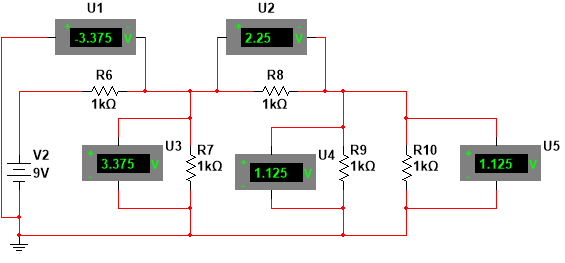
\includegraphics[width=8.075cm, height=3.791cm]{Imagenes/voltajes.png}
	\captionof{figure}{Voltajes de cada elemento.}
	
\end{center}
\begin{center}
	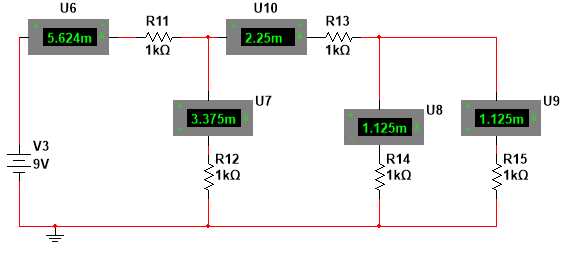
\includegraphics[width=8.075cm, height=3.791cm]{Imagenes/intensidad.png}
	\captionof{figure}{Corrientes de cada elemento.}
	
\end{center}
\begin{center}
	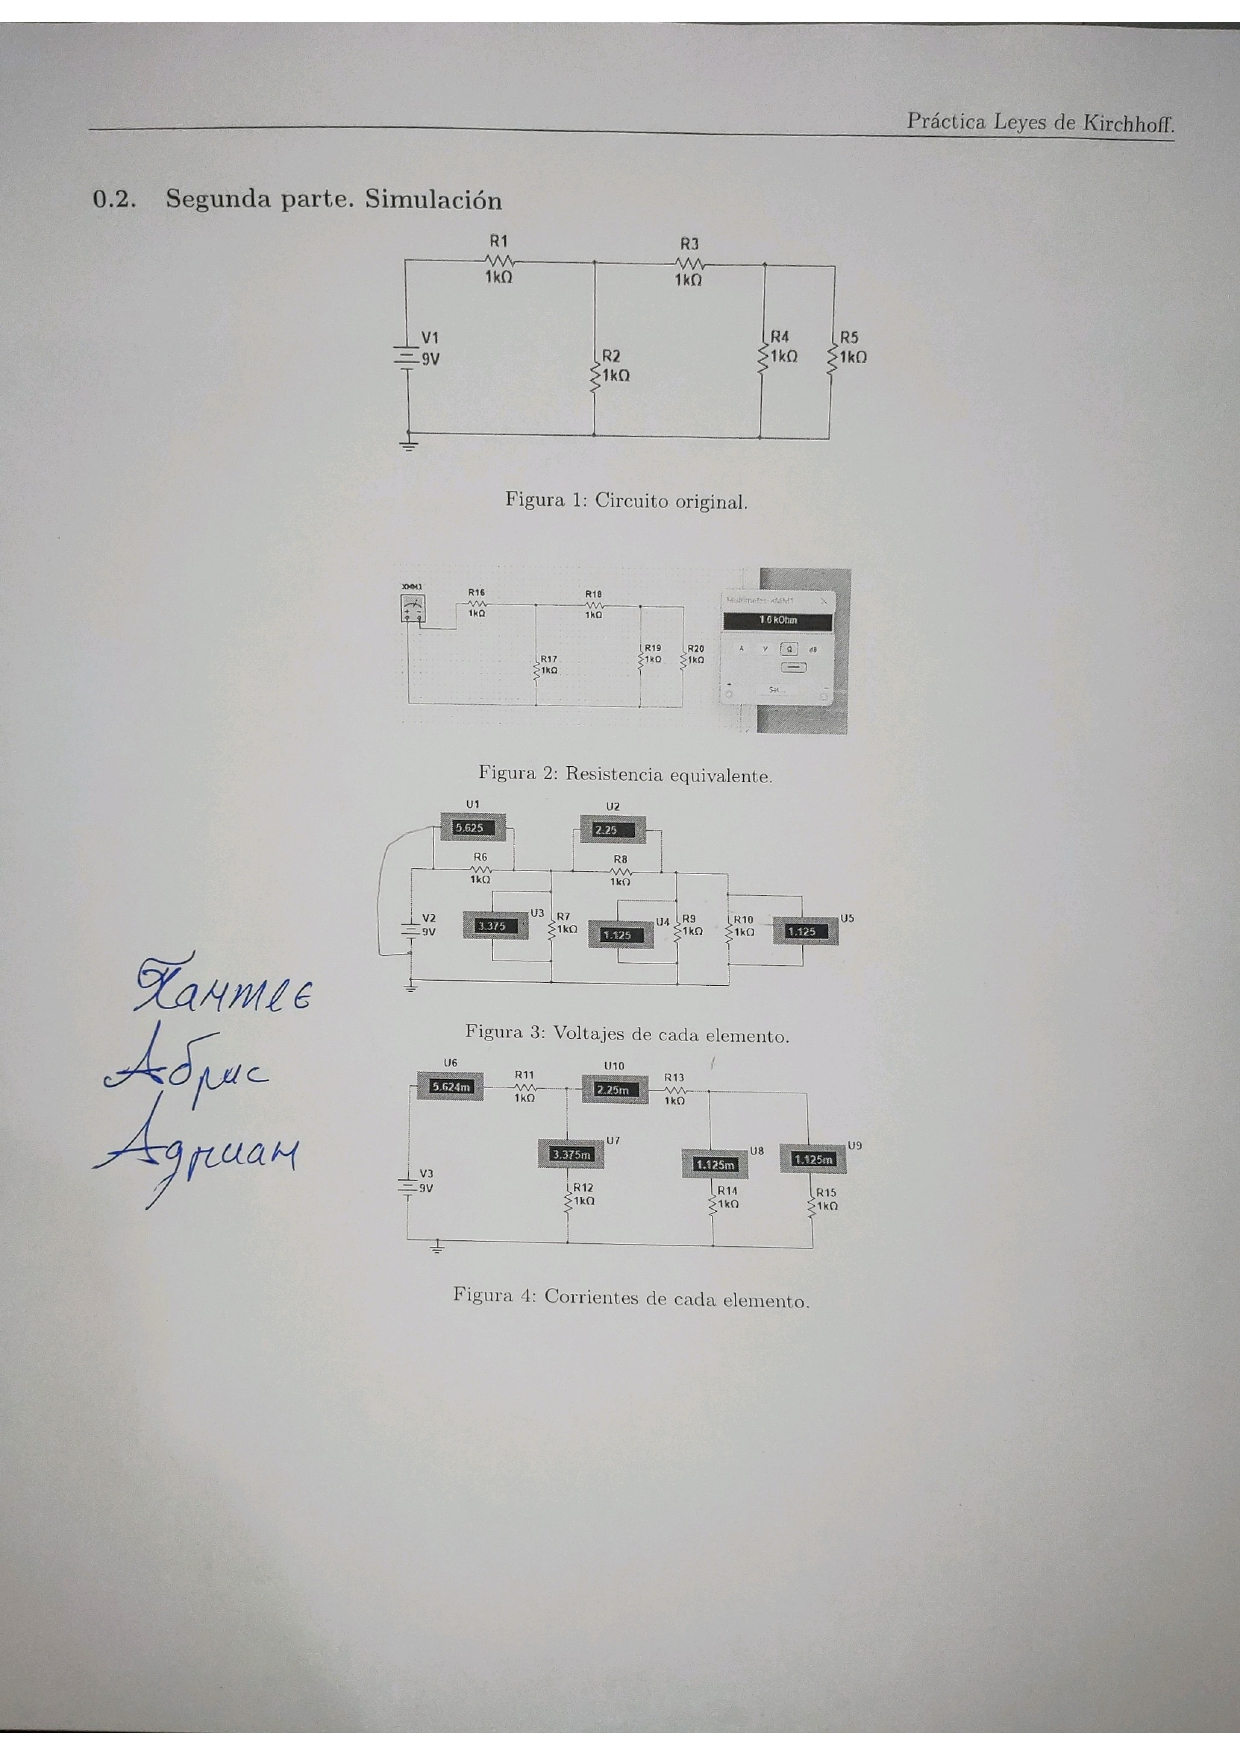
\includegraphics[width=14.5cm, height=18.86cm]{Imagenes/firma.jpg}
	\captionof{figure}{Firma del profe.}
	
\end{center}
\newpage
\subsection{Tercera parte. Mediciones}
\begin{center}
	\begin{adjustbox}{width=340pt}
		\begin{tabular}{|c|c|c|c|c|}
			\hline
			
			 &  & \multicolumn{3}{ |c| }{Mediciones en laboratorio}  \\
			\hline
			 & Valor de resistores en ohms & \multicolumn{3}{ |c| }{$R_{eq} = 1.6k\Omega$}   \\
			\hline
			 &  & Tensión & Corriente & Potencia \\ 
			\hline
			$R_{1}$ &1000 &5.625V &5.625mA &  31.64mW\\
			\hline
			$R_{2}$ & 1000&3.375V &3.375mA &    11.39mW\\
			\hline
			$R_{3}$ & 1000&2.25V & 2.25mA&  5.0625mW\\
			\hline
			$R_{4}$ &1000 &1.125V &1.125mA &1.26mW  \\
			\hline
			$R_{5}$ & 1000 & 1.125V&1.125mA &  1.26mW\\
			\hline
		\end{tabular}
	\end{adjustbox}
\end{center}
\begin{center}
	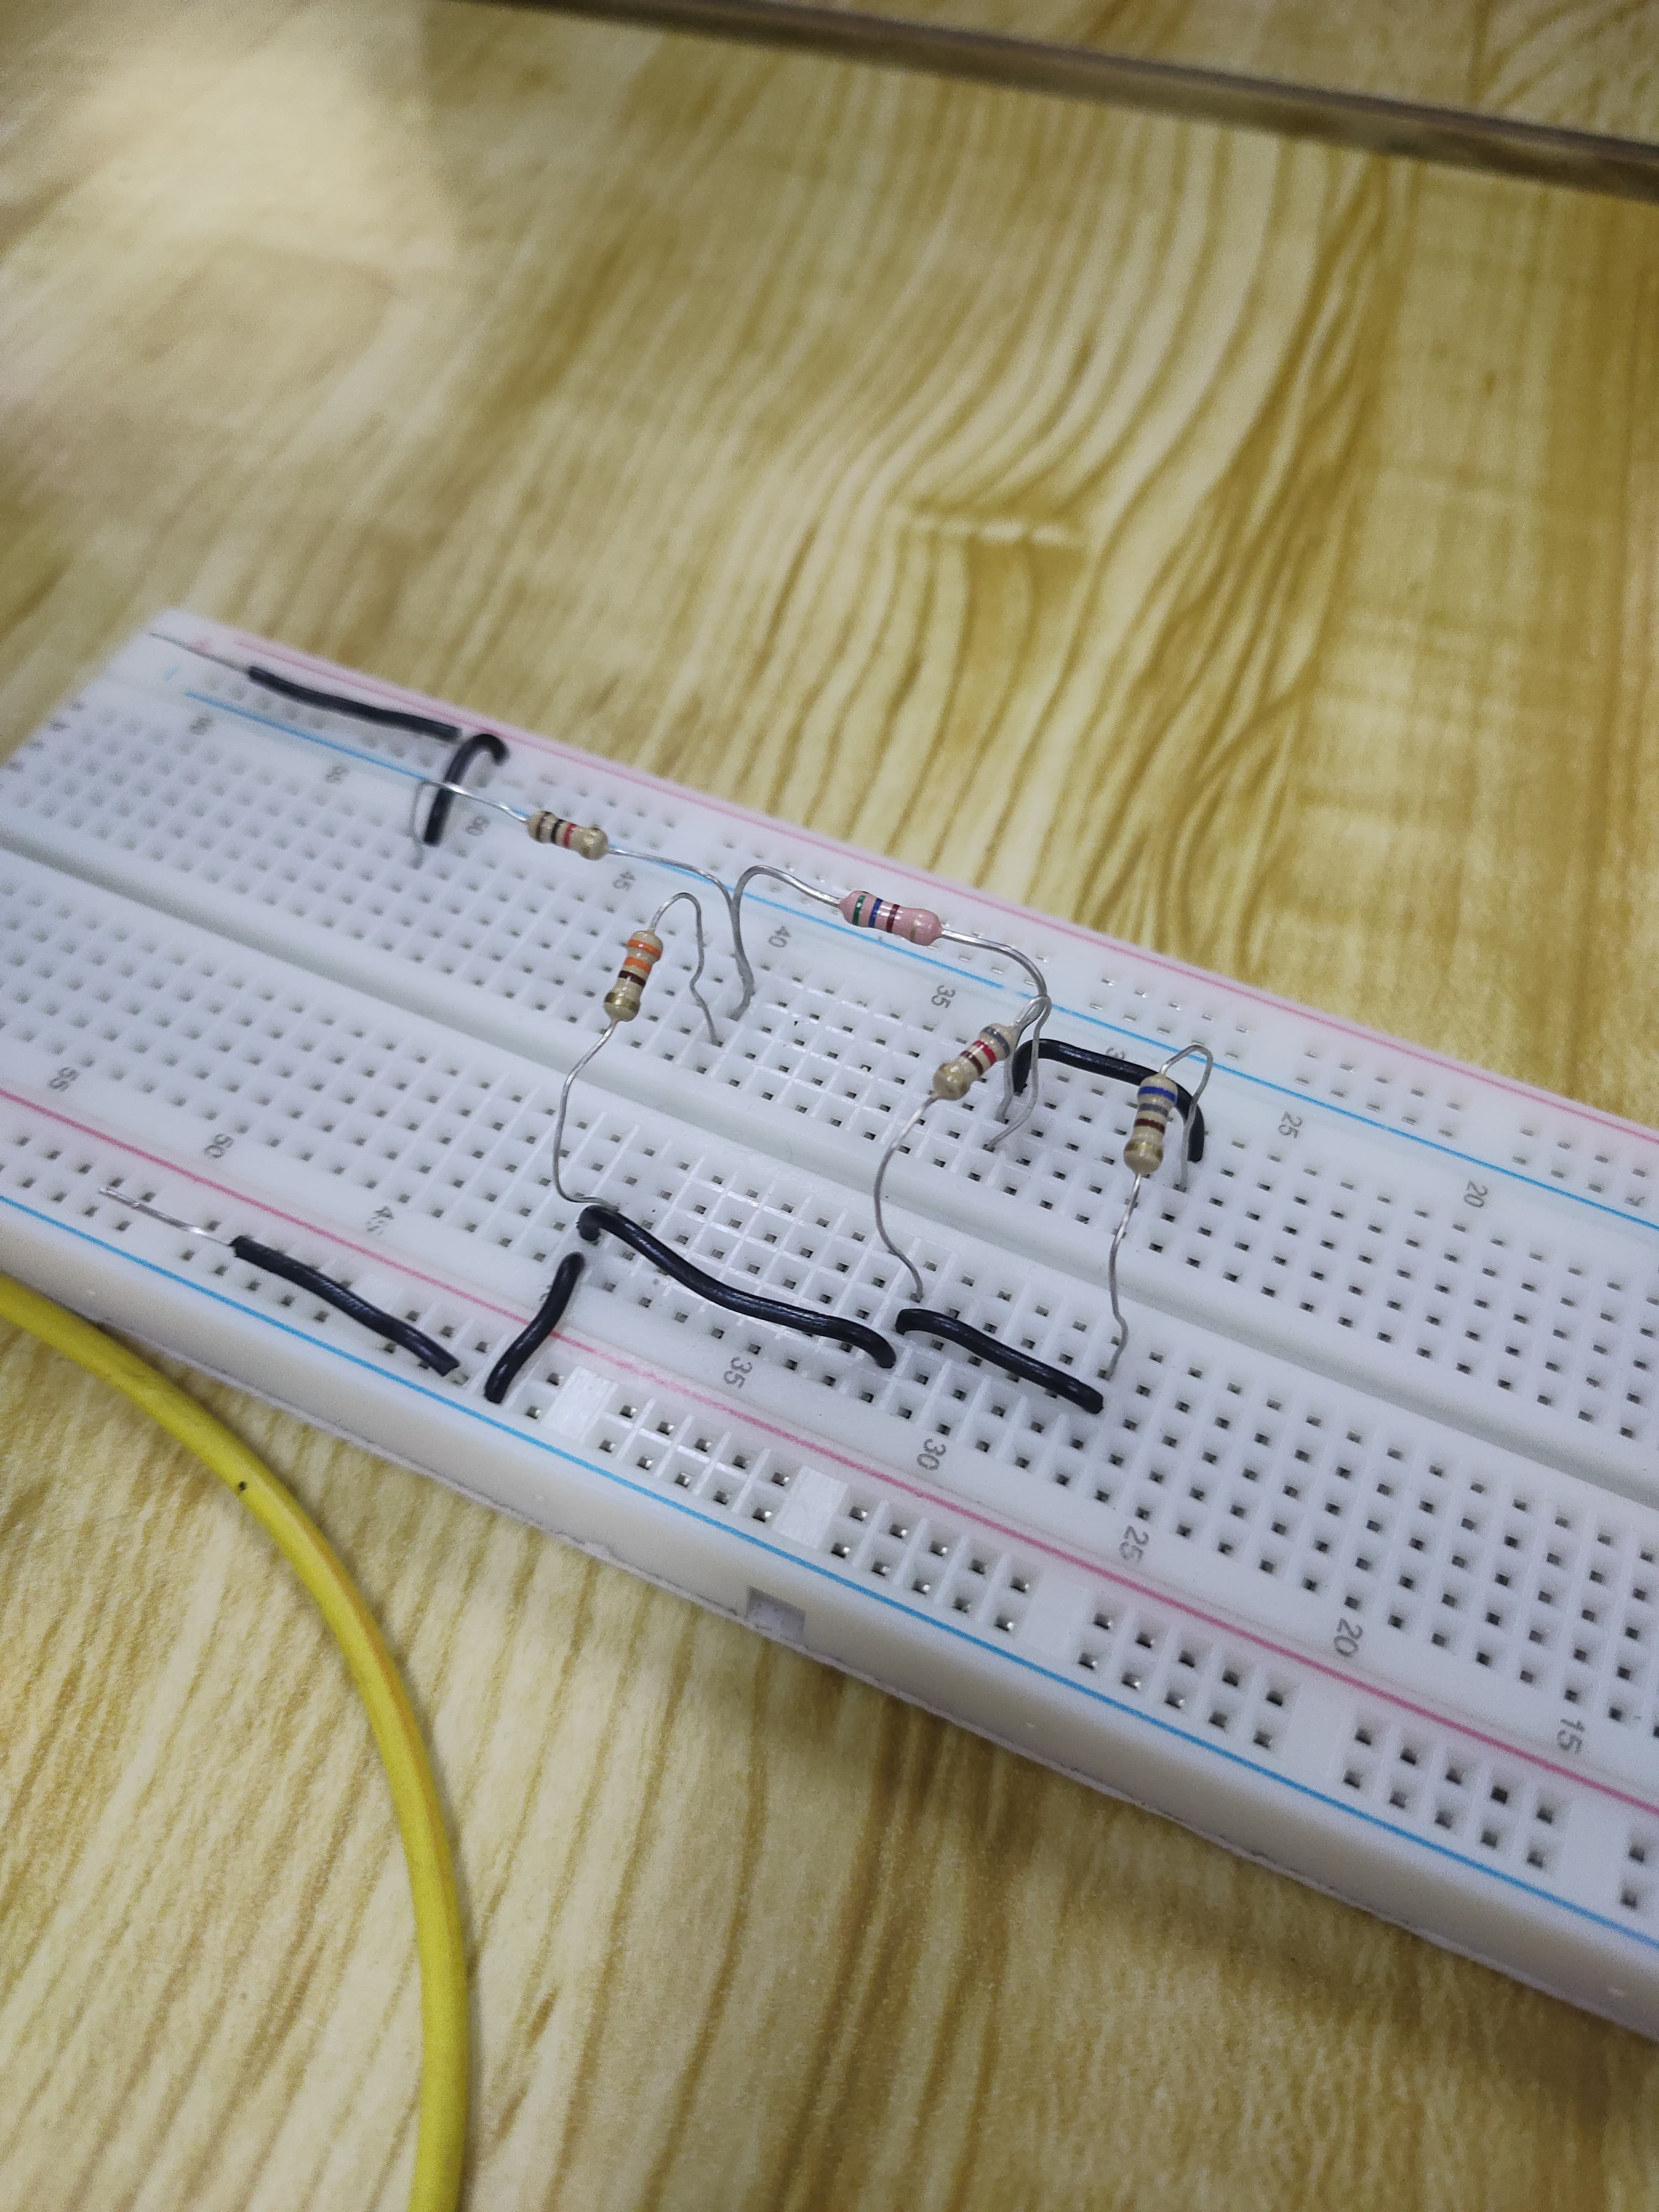
\includegraphics[width=12.5cm, height=16.86cm]{Imagenes/img.jpeg}
	\captionof{figure}{Firma del profe.}
	
\end{center}
\newpage
\section{Tablas}
\subsubsection{Primera parte. Cálculos teóricos}
\begin{center}
	\begin{adjustbox}{width=340pt}
		\begin{tabular}{|c|c|c|c|c|}
			\hline
			
			 &  & \multicolumn{3}{ |c| }{Teoria}  \\
			\hline
			 & Valor de resistores en ohms & \multicolumn{3}{ |c| }{$R_{eq} = 1.6k\Omega$}   \\
			\hline
			 &  & Tensión & Corriente & Potencia \\ 
			\hline
			$R_{1}$ &1000 &5.625V &5.625mA &  31.64mW\\
			\hline
			$R_{2}$ & 1000&3.375V &3.375mA &    11.39mW\\
			\hline
			$R_{3}$ & 1000&2.25V & 2.25mA&  5.0625mW\\
			\hline
			$R_{4}$ &1000 &1.125V &1.125mA &1.26mW  \\
			\hline
			$R_{5}$ & 1000 & 1.125V&1.125mA &  1.26mW\\
			\hline
		\end{tabular}
	\end{adjustbox}
\end{center}


\subsubsection{Segunda parte. Simulación}
\begin{center}
	\begin{adjustbox}{width=340pt}
		\begin{tabular}{|c|c|c|c|c|}
			\hline
			
			 &  & \multicolumn{3}{ |c| }{Simulación}  \\
			\hline
			 & Valor de resistores en ohms & \multicolumn{3}{ |c| }{$R_{eq} = 1.6k\Omega$}   \\
			\hline
			 &  & Tensión & Corriente & Potencia \\ 
			\hline
			$R_{1}$ &1000 &5.625V &5.625mA &  31.64mW\\
			\hline
			$R_{2}$ & 1000&3.375V &3.375mA &    11.39mW\\
			\hline
			$R_{3}$ & 1000&2.25V & 2.25mA&  5.06mW\\
			\hline
			$R_{4}$ &1000 &1.125V &1.125mA &1.40mW  \\
			\hline
			$R_{5}$ & 1000 & 1.125V&1.125mA &  1.40mW\\
			\hline
		\end{tabular}
	\end{adjustbox}
\end{center}





\end{document}
